\label{sec:theory}

\section{Die Programmiersprache Ruby}

Ruby ist eine Programmiersprache, die ab 1993 von Yukihiro Matsumoto entwickelt wurde. Dabei ließ er sich von seinen Lieblingsprogrammiersprachen Perl, Smalltalk, Eiffel, Ada und Lisp inspirieren, um eine neue Programmiersprache zu entwickeln, die sowohl funktionale und imperative Programmierung ermöglicht \citep{ruby_visual_identity_team_about_2011}. 

Eine vollständige Einführung in Ruby zu geben, würde den Rahmen dieser Diplomarbeit sprengen, weswegen ich mich auf die Herausstellung der Hauptmerkmale und Unterschiede zu anderen Sprachen konzentrieren werde, und was die Auswirkungen auf das Testgeschehen sind.

%Dem geneigten Leser seien zum Selbststudium 
% http://tryruby.org/
% .... TODO

\subsection{Einführung in Ruby}
\marginline{
\includegraphics[width=0.8\marginparwidth]{material/ruby.png}
Ruby ist eine Multiparadigma-Sprache}
Ruby ist eine Multiparadigma-Sprache, die Objektorientierung, prozedurale, funktionale und nebenläufige Programmierung unterstützt. Im Gegensatz zu Java ist Ruby wie Smalltalk vollständig objektorientiert. So sind auch alle Datentypen wiederrum Objekte, was auch die primitiven Datentypen wie String und Integer umfasst. 

Ruby ist dynamisch stark typisiert, d.h. dass die Zuweisung des Typs einer Variable zur Laufzeit des Programms geschieht. Der Typ einer Variable ergibt sich damit aus ihrem Wert.

Ruby ist eine interpretierte Sprache, auch Skriptsprache genannt. Dies heisst, dass der Programmcode zur Laufzeit analysiert und ausgeführt wird. 
% TODO Quelle!!

Ruby nimmt für sich in Anspruch, eine Sprache für Menschen, und nicht für Maschinen zu sein. Dies drückt sich durch eine Syntax, die oft laut als englische Sprache gelesen werden kann. 

\setlength{\epigraphwidth}{\marginparwidth}
\marginline{\epigraph{Ruby is simple in appearance, but is very complex inside, just like our human body}{Yukihiro Matsumoto}}
\setlength{\epigraphwidth}{0.8\textwidth}

Im Nachfolgenden einige Beispiele für die Verwendung von Ruby, insbesondere die "`Alles ist ein Objekt"'-Philosophie.

\begin{lstlisting}[language=Ruby,label=Ruby Beispiele,caption=Ruby Beispiele]
 
>> puts "Hello World"
=> Hello World

>> 2.even?
=> true

>> "hallo".upcase
=> "HALLO"

>> Date.today + 2
=> #<Date: 2011-06-30>

>> a = 4 + Math.sqrt(9)
=> 7.0

>> if (0..10).include? a
>>   puts "a liegt zwischen 0 und 10"
>> end
=> a liegt zwischen 0 und 10

\end{lstlisting}

Desweiteren sei die sehr gute Unterstützung bei der Bearbeitung von Strings hervorzuheben. Insbesondere die Regulären Ausdrücke sind denen von Perl beinahe gleichmächtig und fest in die Sprache als Syntaxelement eingebaut.

\begin{lstlisting}
>> match = "2011-06-20".match /(?<year>\d{4})-\d{2}-\d{2}/
>> puts match[:year]
=> 2011
\end{lstlisting}

Auch die Bearbeitung von Arrays und listenähnlichen Strukturen ist sehr bequem, dank der Verwendungsmöglichkeit von anonymen Funktionen, bei Ruby "`Blöcke"' genannt.

\begin{lstlisting}
>> [5,5,7,3].sort
=> [3, 5, 5, 7]

# Es kann auch eine benutzerdefinierte Sortierfunktion
# angegeben werden
>> [ "string",  "rails",  "ruby" ].sort_by{ |item| item.length }
=> ["ruby", "rails", "string"]

# Die Quadratzahlen von 1 bis 5
>> (1..5).map{|element| element * 2}
=> [2, 4, 6, 8, 10]
\end{lstlisting}
Neben einem soliden objektorientierten System, bietet Ruby viele funktionale Aspekte, um die Arbeit mit Arrays und Strings sehr einfach zu gestalten. Wichtig sei auch noch die Fähigkeit der Metaprogrammierung anzumerken.

Im Gegensatz zu Java oder C\# dürfen Klassen zur Laufzeit um Funktionen erweitert, oder alte sogar überschrieben werden. So ist es z.B. möglich, die String-Klasse um eigene Funktionen zu erweitern.

\begin{lstlisting}
>> class String
>>   def remove_whitespace
>>     self.gsub(/\s+/, "")
>>   end
>> end

>> "Dies ist ein Test".remove_whitespace
=> "DiesisteinTest"

\end{lstlisting}

Diese Beispiele sollten als kurzer Einstieg in Ruby dienen, und einen Querschnitt durch die Besonderheiten der Sprache aufzeigen.

Für eine weiter Vertiefung sei das Buch "`Programming Ruby 1.9"' empfohlen, das im Detail auf die neuste Version der Programmiersprache eingeht.

\subsection{Diskussion}

\paragraph{Ruby als Skriptsprache}
Dynamisch typisierte Sprachen, wie Ruby, haben gegenüber klassischen statisch typisierte Sprachen einige Nachteile. Zu allererst wir oft der Geschwindigkeitsnachteil angesprochen, den der Prozess des Interpretierens und das fehlende statische Typsystem verursachen.
Allerdings hat dies in der Regel gravierende Geschwindigkeitsnachteile. Der genaue Faktor variiert extrem, je nach Algorithmus. Ein beliebter Benchmark, shoutout.alioth, vergleicht beliebte Algorithmen der Informatik implementiert in verschiedenen Sprachen miteinander. So ergibt sich z.B. in der Gegenüberstellung von Ruby mit C ein 4-300 fache langsamere Ausführungszeit. Dem gegenüber steht allerdings jeweils nur die Hälfte bis $1/7$ der Menge an Code \citep{computer_language_benchmarks_game_ruby_2011}.

Ein Vorteil des Interpretierens, also der Übersetzung zur Laufzeit, ist eine hohe Plattformunabhängigkeit und ein leichterer Buildprozess, da das Kompilieren entfällt. 
Verfechter dynamischer Sprachen erklären weiterhin, dass diese sich ideal für prototypische Implementierungen eignen, da sich Anforderungen ständig ändern können. Weiterhin hätten Programme dynamischer Sprache eine potenziell hohe Wiederverwendbarkeit und eine höhere Lesbarkeit \citep{meijer_static_2005} \citep{ousterhout_scripting:_1998}.

Desweiteren bleiben Fehler, die der Compiler bereits entdeckt hätte, bis zur Ausführung oder schlimmstenfalls noch länger unentdeckt. Dazu gehören z.B. Tippfehler, bei denen der Wert einer nicht deklarierten Variable ausgelesen wird. Im Gegensatz zu z.B. PHP, wirft Ruby aber dann eine Exception.

Auf das Testen hat dies eine direkte Auswirkung. Viele Meinungen belegen, dass eine dynamisch typisierte Sprache mehr Tests benötigt, als eine statisch typisierte \citep{daniel_spiewak_dynamic_2010}. 



\paragraph{Metaprogrammierung}
Die Fähigkeiten zur Metaprogrammierung von Ruby bieten vielerei Möglichkeiten um Probleme effektiv zu lösen, die andernfalls nur mit erheblichem Aufwand, oder gar nicht zu lösen sind. So verwendet das beliebte Objektrelationale Datenbankframework ActiveRecord Metaprogrammierung, um einfache SQL-Statements zu erstellen.
\begin{lstlisting}
>> Person.find_by_first_name("Stefan")
  Person Load (0.2ms)  SELECT persons.* FROM persons
    WHERE users.first_name = 'Stefan' LIMIT 1
\end{lstlisting}

Die Methode \texttt{find\_by\_first\_name} existiert nicht, und wird zur Laufzeit auf Basis des Namens gebaut.

Auch das sehr beliebte Testframework Rspec, auf das wir später kurz eingehen werden, verwendet Metaprogrammierung, um Testfälle und Zusicherungen wie fast in der englischen Sprache zu formulieren.

\begin{lstlisting}
>> 4.should == 3
RSpec::Expectations::ExpectationNotMetError: expected: 3
\end{lstlisting}

All diese Methoden können, richtig angewendet, zur Verbesserung der Lesbarkeit der Programme, und damit zur Erhöhrung der Wartbarkeit, führen.
Falsch angewendet stellen sie jedoch eine Gefahr da. Beim Verwenden von externen Bibliotheken, oder in einem großen Entwicklerteam können dadurch kuriose Fehler auftreten die nur sehr schwer zu finden sind. Potenziell jedes Quelltextfile kann jede Klasse zur Laufzeit verändern, ohne dass es eine Warnung gibt. Umgehen kann man dieses Problem bestenfalls durch das konsequente Einordnen in Namensräume, bei Ruby Module genannt.
%TODO Quelle?

\paragraph{Schlussfolgerung}

Die Verwendung von Ruby und anderen dynamischen Sprachen birgt durchaus Risiken, die zu beachten sind. Falls man diese Risiken im Kopf behält, und die Möglichkeiten der Sprache nutzt, um die Lesbarkeit zu verbessern, sind sie gerechtfertigt. Gerade bei der Entwicklung kleinerer Entwicklerteams oder Projekten mit engem Budget können dynamische Sprachen ihre Vorteile ausspielen, da sie eine eine schnellere Entwicklung ermöglicht. Im Gegensatz zu den meisten auf C basierten Sprachen, ist die Syntax von Ruby äußerst leserlich, da nur wenige Sonderzeichen verwendet werden. Auch biete Ruby mehr Funktionalität pro Programmzeile, da die Deklaration entfällt und es viel sogenannten syntaktischen Zucker gibt. Auch dies kann, richtig angewendet, der Lesbarkeit zuträglich sein.
% TODO QUelle hier was?
\epigraph{Sometimes people jot down pseudo-code on paper. If that pseudo-code runs directly on their computers, it's best, isn't it? Ruby tries to be like that, like pseudo-code that runs. }{Yukihiro Matsumoto}


\subsection{Ruby on Rails}

Für das Projekt IT-jobs-und-stellen.de soll das Webframework Ruby-on-Rails verwendet werden. Rails wurde 2006 von der Firma 37signals unter der Leitung von David Heinemeier Hansson entwickelt und erlangte seitdem eine wachsende Popularität. Rails inspirierte viele andere Frameworks, wie z.B. cakePHP, Groovy on Grails, Symfony und ASP.NET MVC.

\marginline{
\includegraphics[width=0.8\marginparwidth]{material/rails.png}}
Viele professionelle Websites, die meist als Startup begannen, setzen bis heute auf Rails. Darunter z.B. Yellow Pages, die Gelben Seiten der USA, Github, eine sehr beliebte Community für OpenSource Programmierer,  Groupon, dem führenden Unternehmen bei Online-Gutscheinen und XING, einer deutschen Online-Community für Business-Kontakte.
% TODO http://rubyonrails.org/applications

%TODO Quelle http://www.businessinsider.com/heres-why-ruby-on-rails-is-hot-2011-5
Im Folgenden werden die Grundzüge von Ruby on Rails näher erläutert.

\subsubsection{Konzepte von Rails}

Rails ist ein Webframwork, das auf dem Model-View-Controller-Pattern basiert, welches eine 3-schichten Architektur darstellt. Jede Schicht hat fest definierte Aufgaben. Diese bilden normalerweise ein Dreigespann, bei Rails "`Ressource"` gennannt. Im folgenden werden die Schichten kurz erläutert, und am Beispiel einer Ressource "'Job"` 
\begin{description}
 \item[Model] In Klassen dieser Schicht werden Zugriffe auf die Persistenz vorgenommen. Meist geschieht dies durch Ausführung von SQL-Befehlen. Innerhalb von Rails ist dies aber meist nicht notwendig, da das ORM\footnote{Objektrelationale Framework} ActiveRecord häufig verwendete SQL-Befehle abstrahiert. Auch die Geschäftslogik soll per Definition zu großem Teil in dieser Schicht erfolgen.
 
 Für einen Job ist das ein Modell, welches die Datenbanktabelle "'jobs"` anspricht, und z.B. die Attribute "'titel"`, "'datum"` und "'beschreibung"` besitzt. Dabei können auf diesem Level auch datenbankunabhängige Constraints definiert werden, z.B. dass ein Job nur dann gespeichert werden soll, wenn der titel mindestens 20 Zeichen lang ist, und das Datum mindestens das heutige ist.
 % TODO Fat models thin controllers
 \item[Controller] Klassen dieser Schicht vereinigen Methoden, die von außen per HTTP erreichbar sind. Diese Methoden kommunizieren mit den korrespondierenden Models und bestimmen, welche View im einzelnen ausgeliefert wird. Weitere Funktionen eines Controllers sind Authentifizierung und Autorisierung (Wer darf was).\\
 Standardmäßig stellt Rails die CRUD\footnote{Create Read Update Delete}-Operationen bereit, welche in Form eines REST\footnote{Representational State Transfer die HTTP-Methoden GET, POST, PUT, DELETE werden in Kombination mit einem definierten URL-Schema direkt auf die Aktionen \texttt{Auflisten, Anzeigen, Bearbeiten, Löschen, Neu anlegen} gemappt.
 \url{http://en.wikipedia.org/wiki/Representational_State_Transfer}}
 \item[View] Eine View ist in der Regel ein Stück HTML Code welches einem Model zugeordnet ist, das bei einer bestimmten Aktion dem Clienten ausgeliefert wird. Neben HTML ist auch Javascript oder XML eine mögliche Auslieferungsform.\\
 Für den Job wäre das eine View für die Liste aller Jobs, einen Job im Detail anzeigen sowie das Formular zum Anlegen und Bearbeiten eines Jobs.
 \end{description}
 \begin{figure}[h]
  \centering
  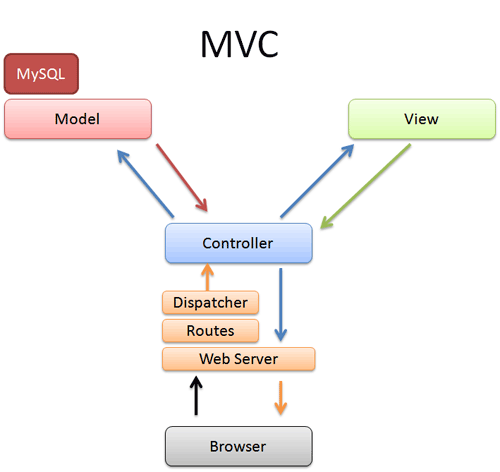
\includegraphics[width=0.7\textwidth]{./material/mvc-rails.png}
  % mvc-rails.png: 500x472 pixel, 72dpi, 17.64x16.65 cm, bb=
  % SOURCE  
  \caption{MVC Modell von Rails}
  \caption*{Quelle: \href{http://betterexplained.com/articles/intermediate-rails-understanding-models-views-and-controllers/}{betterexplained.com}}
 \label{fig:mvcrails}
\end{figure}
In Abbildung \ref{fig:mvcrails} ist der Ablauf einer Anfrage an den Server dargestellt. Die Anfrage des Browsers an die Website \texttt{http://localhost/jobs/12} wird über den Webserver, z.B. Apache2, an die Railsanwendung gestellt. Innerhalb von Rails wird dieser Anforderungsstring anhand der Routen, die die Anwendung anbietet, gematcht. In unserem Falle würde \texttt{/jobs/12} auf den Controller jobs aufgelöst werden. Innerhalb dieses Controllers wird eine Methode (Aktion) show erwartet.
Diese Methode wird nun ihrerseits eine Anfrage an das Model Job stellen, den Job mit der ID 12 aus der Datenbank zu holen. Danach wird ein HTML Template zur Detailanzeige des Jobs generiert.

\setlength{\epigraphwidth}{\marginparwidth}
\marginline{\epigraph{Ruby on Rails is a breakthrough in lowering the barriers of entry to programming. Powerful web applications that formerly might have taken weeks or months to develop can be produced in a matter of days.}{Tim O'Reilly, Founder of O'Reilly Media}}
\setlength{\epigraphwidth}{0.8\textwidth}

Neben diesem architektorischen Konzept verfolgt Rails noch andere Strategien, um das Entwickeln produktiver zu gestalten.
\begin{description}
 \item[Convention over Configuration] Rails ist so konzipiert, um als Framework komplett out-of-the-box zu funktionieren. Außer die Datenbankeinstellung wird keine Konfiguration im Vorderfeld benötigt. Diese Methodology zieht sich auch durch das Ökosystem durch. Die meisten externen Bibliotheken, bei Ruby Gems genannt, funktionieren bereits nach wenigen Kommandos. Dies macht das prototypische Entwickeln äußert effektiv. Weiterhin ist die Struktur eines Railsprojektes extrem fest definiert. So gibt es u.a. einen Ordner "'app"` mit den Model, Controller und View Dateien und einen Ordner "'test"`, der wiederrum in "'unit"`, "'functional"`, "'integration"` und "'performance"` unterteilt ist. So finden sich Railsprogrammierer auch in fremden Projekten sofort zurecht.
 \item[Don't repeat yourself (DRY)] Hier ist das Ziel, die Duplikation soweit wie möglich zu reduzieren, und das ständige Auslagern und Refaktorisieren des Codes, um bei Änderungen nur an einer Stelle ansetzen zu müssen. Ein weiteres Beispiel ist die Definition der Spalten des ORMs. Im Gegensatz zu anderen ORM-Frameworks ist diese bei Rails nicht notwendig. Rails erstellt automatisch Getter und Setter für die in der Datenbank definierten Tabellenspalten.
 \item[REST] Representational State Transfer ist Software-Architektur für HTTP-WebServices. Dabei werden neben den Standard HTTP Methoden GET und POST auch die selten benutzen Verben DELETE und PUT verwendet, um Aktionen auf einer Ressource zu definieren. Das Ziel ist ein sehr einfaches Design der URLs. Hier folgt die Auflistung der vier CRUD Operationen plus Auflistenvon REST am Beispiel einer Ressource "'jobs"` eines Webservice
 \begin{description}
  \item[GET /jobs.html] Auflisten aller Jobs, Ausgabe als HTML Format
  \item[GET /jobs/12.xml] Job mit der ID 12 anzeigen, Formatiere als XML
  \item[POST /jobs] Einen Job anlegen. Alle benötigten Parameter, wie Titel, Beschreibung oder Datum sollten im POST-Body der HTTP-Anfrage enthalten sein
  \item[PUT /jobs/12] Den Job mit der ID 12 aktualisieren. Die Eigenschaften, die aktualisiert werden, müssen wiederrum als Parameter mit übergeben werden
  \item[DELETE /jobs/12] Lösche den Job mit der ID 12
  \end{description} 
 Rails macht das Arbeiten im Kontext dieser Architektur sehr einfach, und es gilt als die bevorzugte Methode in der Community, APIs zu bauen. 
 \item[Codegeneratoren] Rails bietet viele Codegeneratoren an, um schnell benötigte Klassen und Datenbanktabellen anzulegen. Im Railsprojekt reicht z.B.:
\begin{lstlisting}
rails generate scaffold job title:string description:text \
  start_date:datetime active:boolean user:references
\end{lstlisting}
  Damit wird das Model Job, eine Erstellung der Tabelle "'jobs"`, ein Controller "'jobs"` mit den REST-Standardaktionen und entsprechenden Beispielviews, sowie Testfälle für Unit- und Funktionale Tests angelegt. Weiterhin sei zu bemerken, dass durch die Anweisung \texttt{user\:references} eine Spalte \texttt{user\_id} angelegt wird und eine 1:n-Beziehung zum Modell "'user"` hergestellt wird.
 \item[Full-Stack Webframework] Rails bringt out-of-the-box alles mit, was zur Webentwicklung benötigt wird. Im Gegensatz zu anderen Webframeworks wurde für Datenbankanbindung, Templatesystem, Javascriptframework, Testframework und Webserver-API bereits eine Vorauswahl getroffen. Im aktuellen Rails 3.1 sind dies ActiveRecord, ERB, JQuery, sowie Test::Unit und Rack. Die meisten dieser Teil-Frameworks lassen sich zwar leicht austauschen, Rails selbst aber proklamiert "'opinionated"`, also rechthaberisch/eigensinnig, zu sein, und den Entwickler Standards vorzugeben \citep{david_heinemeier_hansson_railsconf_2011}.
 \epigraph{Rails will have strong defaults. They might change over time but Rails will remain opinionated.}{David Heinemeier Hansson, Begründer von Rails}
\end{description}

Eine Einführung und Programmierung in Rails soll nicht Bestandteil dieser Diplomarbeit werden. Für eine weitere Einarbeitung seien die folgende Quellen insbesondere empfohlen:
\begin{description}
 \item[Rails for Zombies] Dies ist ein moderner, interaktiver Onlinekurs. Greg Pollack und das Team von RailsEnvy verpackt die Lektionen in humorige interaktive Lernerfahrungen. Jeweils eingeleitet durch ein Video muss der Teilnehmer Aufgaben direkt im Sourcecode lösen. Mithilfe dieses Kurses gelang es mir, meinen Arbeitskollegen einen guten Überblick über Rails zu verschaffen. Die Teilnahme ist kostenlos.\\
 \url{http://railsforzombies.org/}
 \item[Agile Webdevelopment with Ruby on Rails] Das quasi-Standardwerk. Wird meist parallel mit einer neuen Rails-Version in einer neuen Auflage gedruckt, aktuell die Dritte \citep{ruby_agile_2009}.
 \item[Rails Guides] Die von Ruby-on-Rails herausgegebenen "'Rails Guides"` sind eine gut strukturierte, kostenlose Online-Dokumentation, die nahezu alle Aspekte von Rails beleuchten.\\
 \url{http://guides.rubyonrails.org/getting_started.html}
 \end{description}



\subsubsection{Diskussion}
Nach einem kurzen Überblick über Rails, sollen nun die Eigenschaften des Frameworks diskutiert werden, und welche Auswirkungen sich dadurch auf das Testen ergibt.
\paragraph{Vorteile}
%TODO  a lot

Dank der Modularität können als Persistenzgrundlage sowohl relationale Datenbank, wie MySQL, SQlite und Oracle, aber auch andere Formen, wie NoSQL-Datenbanken transparent verwendet werden. Dank einer einfach zu verstehenden Syntax, ist das Schreiben von SQL in 95\% der Fälle überflüssig und zudem auch sicherer. Hier ein Beispiel, wie das Anlegen und Auslesen einer Instanz "'Vertragsart"` erfolgt. Parallel dazu ls Kommentar die SQL Kommandos, die ActiveRecord im Hintergrund ausführt.
\begin{lstlisting}
c = ContractType.new
c.name = "Vollzeit"
c.save
=> false
#  SQL (0.1ms)  BEGIN
#  SQL (0.3ms)  SELECT 1 FROM `contract_types` 
#     WHERE (`contract_types`.`name` = BINARY 'Vollzeit') LIMIT 1
#  SQL (0.1ms)  ROLLBACK
>> c.errors
=> {:name=>["Name bereits vorhanden. Der Name muss einmalig sein"]}
>> c.name = "Praktikum"
>> c.save
=> true
#  SQL (0.1ms)  BEGIN
#  SQL (0.4ms)  SELECT 1 FROM `contract_types` 
#     WHERE (`contract_types`.`name` = BINARY 'Praktikum') LIMIT 1
#  SQL (0.4ms)  describe `contract_types`
#  AREL (0.4ms)  INSERT INTO `contract_types` (`name`) VALUES ('Praktikum')
#  SQL (7.1ms)  COMMIT
\end{lstlisting}
Hierbei ist auch schön zusehen, wie in Rails standardmäßig Transaktionen verwendet werden. Auch sieht man, wie eine Validierung funktioniert. Für das Modell VertragsArt wurde eine Einmaligkeit des Attributs name vereinbart. Dies prüft Rails vor dem Speichern und bricht das Speichern ab, falls eine Prüfung fehlschlug.

Die Implementation dieser Prüfung ist denkbar einfach.
\begin{lstlisting}
class ContractType < ActiveRecord::Base
  validates :name, :uniqueness => true, :presence => true
  
  has_and_belongs_to_many :jobs
end
\end{lstlisting}
Wir vereinbaren so, dass das Attribut Name einmalig sein muss (uniqueness), und ausgefüllt sein muss (presence). Die andere Zeile mit has\_and\_belongs\_to\_many definiert eine n:m Beziehung mit dem Modell Job, d.h. ein Job hat mehrere Vertragsarten. Der Rest geschieht dann durch Metaprogrammierung.

Mit minimalem Code lassen sich so komplexe Probleme abbilden. Dies macht Rails zu dem hochproduktivem Framework, als das es entwickelt wurde.
\epigraph{I needed to be way more productive...}{David Heinemeier Hansson}
%TODO Quote

Rails bietet eine gute Ausgangsbasis um sichere Websoftware zu entwickeln. Das Verwenden eines Datenbankframeworks macht SQL-Injections unmöglich. 
Cross-Site-Scripting
Cross-Site-Request-Forgery und Session-Angriffe werden erschwert, da Session und Cookie Variablen standardmäßig verschlüsselt werden.
Durch die Verwendung des

% SQL Injection
% Tower of Babel

\paragraph{Nachteile}
Interaktion mit Legacy-Software ist nicht immer möglich. ActiveRecord reserviert ein paar Spaltennamen, wie \texttt{type} und  class. Eine Benennung der Spalten sollte der Ruby-Namenskonvention entsprechen, also nur Buchstaben Zahlen und Unterstriche enthalten. Ansonsten können die Spalten nur über Umwege angesprochen werden.

\paragraph{Performance} Oft wird angeführt, dass Ruby als Skriptsprache und Rails als darauf aufbauendes Framework eine schlechte Performance hat, und dadurch ungeeignet für große Webanwendungen ist.
%TODO QUelle, wer sagt das?

%TODO Benchmark, Diskussion zur Architektur

Anderseits gibt es Anzeichen dafür, dass eine clevere Architektur und Caching für skalierende Anwendung entscheidender ist, als die letztendliche Ausführungszeit.

Das dies möglich ist, zeigen z.B. Groupon, der führende Online-Coupon-Anbieter mit mehr als 50 Mio Abonnenten und 
%TODO http://www.socialshopping.com/Groupon/news/Groupon-hits-50m-Subscribers-Shopping-site-sensation-201101210398/
Twitter, die jeweils Rails verwenden.
%TODO Quelle Rails applications

\paragraph{Rails und Tests}
Rails bietet ausgezeichnete Vorraussetzungen zum Softwaretest. Dafür sprechen, dass...

\begin{itemize}
 \item benötigte Bibliotheken bereits mitgliefert werden,
 \item die Verwendung stark erleichtert wird, da Rails beim Nutzen der Codegeneratoren analoge Testdateien gleich mitgeneriert,
 \item das Rails Ökosystem eine Vielzahl von Testtools bereitstellt, u.a. Rspec (BDD\footnote{Behavior Driven Development - Siehe später}-Testframework), Rcov (Testabdeckung), diverse Mockbibliotheken (mocha, FlexMock, RR, Rspec Mocks), Tools zum Generieren und Bereitstellen von Testdaten (Fixtures, Factories, Faker) und Codemetriken (metric-fu)
 \item das Testen in der Rails Community einen sehr hohen Stellenwert hat, so dass die meisten Bibliotheken und Plugins getestet werden
 %TODO Quelle
\end{itemize}

Dabei werden mehrere verschiedene Testarten unterstützt und definiert.
\begin{description}
 \item[Unittests] oder Modeltests. Zielstellung: Hier wird die Logik einer Modelklasse untersucht\\
 Testziel: alle (komplexeren) Methoden die das Modell anbietet. Am Beispiel Job kann das die Aussage sein, wann ein Job gültig ist, d.h. welche Bedingungen für die einzelnen Attribute gelten sollen.\\
 Testart: Whitebox
 \item[Funktionale Tests] Untersuchungsgegenstand sind die Controller, also die Schnittstellen zum Nutzer. \\
 Testziel: Getestet wird meist der Arbeitsablauf innerhalb eines Controllers, also Weiterleitungen, Benachrichtigungen und welches Template gerendert wird.\\
 Testart: Whitebox
 Es können auch oberflächliche View-Tests unternommen werden, also die Aussage ob ein bestimmtes HTML-Element auf der Seite zu sehen ist.
 \item[Integrationstests] es wird ein Browser simuliert der von außen auf die Applikation zugreift
 Zielstellung: Testen komplexer Interaktionen zwischen verschiedenen Teilen der Software\\
 Beispiel: Ein User loggt sich ein und legt einen neuen Job an\\
 Testart: Graybox oder Blackbox
 \item[Performanz-Tests] Eine Testart, die alle Methoden aus Unittests und Funktionalen Tests beinhaltet\\
 Zielstellung: Herausfinden von Performanz-Flaschenhälsen in allen Ebenen. \\
 Beispiel: Es werden 1000 Jobs generiert und geprüft, ob die Anzeige schnell genug läuft\\
 Testart: Graybox
\end{description}
    

\section{Softwaretests}

\subsection{Warum testen}

(Softwarefehler) \url{http://www.nfranze.de/download/Diplomarbeit_Nico_Franze.pdf}
  Zusammenfassende Begriffsdefinition

\subsection{Arten von Tests}

\subsection{Testtools in Ruby}
\subsubsection{Test::Unit und Minitest}
Test::Unit (Ruby 1.8.7) und Minitest (1.9.2) sind die Testbibliotheken, die Ruby standardmäßig mitbringt. Beide basieren auf dem xUnit, bzw. SUnit Design von Kent Beck, und sind für Nutzer von JUnit oder NUnit leicht nachvollziehbar.

Für eine zu testende Klasse wird eine analoge Testklasse erstellt. Diese trägt per Definition denselben Namen wie die zu testende Klasse mit einem "`test"' am Anfang. Um z.B. eine Klasse "`job"' zu testen, wird eine Datei \texttt{test\_job.rb} (Ruby Standard) oder \texttt{job\_test.rb} (Rails Standard) erstellt. Dort wiederrum wird eine Klasse mit Namen \texttt{TestJob} definiert. 

Ein Beispieltest sieht z.B. so aus:
\begin{lstlisting}
require "job"

class TestJob < Test::Unit::TestCase
  def setup
    @job = Job.create
  end
  
  def teardown
    Job.delete_all
  end
  
  def test_job_exists
    @job.title =  "Ruby on Rails Entwickler
    @job.add_location_to_title( "Dresden")
    
    assert_equal( "Ruby on Rails Entwickler in Dresden",  Job.first.title)
  end
end
\end{lstlisting}
Unsere Klasse TestJob erbt von der TestUnit Basisklasse. Sie beinhaltet die Methoden "`setup"' und "`teardown"', die jeweils vor, respektive nach jedem einzelnen Testfall aufgerufen werden.
In der Setup-Methode nehmen wir z.B. das Anlegen eines Jobs vor, in der Teardown Methode löschen wir alle Jobs in der Datenbank, um einen sauberen Test zu gewährleisten

Danach können nun beliebig viele Testmethoden folgen, deren Namen mit \texttt{test\_} beginnen müssen.
Jede Testmethode besteht in der Regel aus einer Initialisierung (kann in die setup-Methode ausgelagert werden), der Ausführung einer zu testenden Aktion und dem Prüfen der danach geltenden Eigenschaften mittels Assertions. Diese Zusicherungen sind Prädikate die oft Gleichheit oder Boolsche Rückgabewerte prüfen.

%TODO Weitere Prädikate erwähnen

Rails erledigt das Anlegen und Löschen von Testdaten selbständig. Diese werden als Fixtures bezeichnet und extern definiert. Alternativ ist der Einsatz sogenannter Factories möglich, um schnell Objekte mit bestimmten Eigenschaften zu erstellen. In jedem Fall setzt Rails die Datenbank nach jedem einzelnen Test zurück.


\subsubsection{Rspec}
\subsubsection{Cucumber}

\section{Testgetriebene Entwicklung}
Testgetriebene Entwicklung, im Englischen Test-Driven-Development (TDD) wurde erstmalig von Kent Beck 2003 im Detail erläutert. Zuvor war die Technik "`Test-First"' aber schon seit 1999 im Kontext von Extreme Programming (XP) bekannt.
%TODO Quelle: "Extreme Programming". Computerworld. Retrieved January 11, 2011.
%TODO Quelle: Beck, K. Test-Driven Development by Example, Addison Wesley, 2003
Damit wurde aus der Entwicklungs-Methode "`Test-First"' ein Software-Entwicklungsprozess. 

Im Folgenden werde ich diesen Prozess näher beleuchten und am Beispiel von Ruby on Rails typische Testwerkzeuge aufzeigen. \subsection{Motivation}
  Das Erstellen einer gut abdeckenden Test-Suite für ein jedes größeres Softwareprojekt ist eine wichtige Vorraussetzungen um interne Qualitäten, wie Wartbarkeit und Zuverlässigkeit zu aktivieren. TDD soll nicht dazu dienen, die Software zu verifizieren. Dies ist aber ein positiver Nebeneffekt. Das Hauptziel ist es, den Code in Einklang mit dem Test zu schreiben, so dass der Test den Code antreibt (Test drives thes code). Der messbare Effekt davon, ist ein gut-testbarer Code, welcher in der Regel auch ein gut-wartbarer und verständlicher Code. Bad-Smells, wie God-Methode und geringe Kohäsion, werden schon im Keim erstickt werden, da sie selbst nur äußerst schwer zu testen sind.
  
  
  %Psychologische...
  % Zuversicht
  TDD hat auch eine psychologische Motivation.
  In Abbildung \ref{} ist ein Einflussdiagramm zu sehen, welches vereinfacht Zusammenfänge darstellen soll. Ein direkter Pfeil zeigt eine direkte proportionale Abhängigkeit, ein Pfeil mit einem Kreis eine indirekt proportionale Abhängigkeit. In diesem Diagramm soll der Zusammenhang zwischen psychischen Druck auf den Programmier, Testen und Defekte visualisiert werden. Druck führt somit zu weniger Tests, weniger Tests zu mehr Fehlern und diese wiederrum zu höherem Druck. Dieser klassische Teufelskreis der Softwareentwicklung, der gerade zum Ende eines Entwicklungsprozesses auftritt, soll durch TDD effektiv verhindert werden. 
  % TODO Figure A.5 
  TDD fördert die Entwicklung in kleinen Schritten, und ermöglicht durch bestande Tests kleine "`Belohnungen"' für den Programmierer. Dadurch ist es leichter einen gewissen Arbeitsrhythmus zu erhalten, was stellenweise dem "`Flow"'\footnote{Schaffen-, Tätigkeitssrausch}  ähnelt oder diesen strukturiert ergänzen kann.
  % TODO http://www.agilecoachjournal.com/post/Test-Driven-Development.aspx
  
\subsection{Ablauf}
  Ziel ist es, vor der Implementation eines Codes, einen Unittest zu implementieren. Davon ausgehend soll der geringstmögliche Code implementiert werden, damit der Test besteht. Zum Schluss wird refaktorisiert, bei TDD auch als Designphase genutzt.
  
  %TODO Abbildung mit Beschreibung
  Im Ganzen sind das also die Phasen:
  \begin{enumerate}
   \item Schreibe einen Test von dem Feature, das als nächstes entwickelt werden möchte\\Oder von dem Test, der als nächstes auf der Liste steht
   \item Red: Führe alle Tests aus, um sicherzugehen, dass der Test fehlschlägt. Andernfalls ist der Test überflüssig.
   \item Green: Nachdem der Test fehlschlägt, implementiere nun den leichtesten Code, der den Test besteht\\
   Dies kann ausdrücklich auch eine Fake-Implementierung sein. Wichtig ist, dass diese Phase so schnell wie möglich verlassen wird.
   \item Refactor: Nachdem der Test bestanden wird, folgt nun die \textbf{wichtigste Phase}, die Refaktorisierungsphase.\\
   Da wir bereits einen Test haben, der unser gewünschtes Systemverhalten widerspiegelt, können wir gefahrlos refaktorisieren, d.h. im Einzelfall Duplikation eleminieren. In dieser Phase findet das Design des Codes statt. Man macht sich Gedanken, wie die vorhanden Klassen optimal refaktorisieren können, um Code-Smells zu eleminieren.
  \end{enumerate}
  
  Jeder Unittest soll prinzipiell nur eine Eigenschaft testen, die Entwicklung erfolgt also in kleinen Schritten. Dies hat direkte Auswirkungen auf die zu entwickelnden Objekte und Methoden, die ebenfalls übersichtlich werden sollen, und somit dem Funktionsbegriff, eine Methode für eine Aufgabe und erweitert eine Klasse für eine Aufgabe, gerecht werden.
  
  
  Das ganze lässt sich auch in den übergeordneten Prozess zum Entwickeln eines Features einordnen.
  %RSPEC Buch macht das vor, Noch mal schauen, evtl alles Käse was ich hier geschrieben habe
  \begin{enumerate}
   \item Schreibe einen Integrations/Akzeptanztest um das aktuelle Feature zu implementieren
   \item Nach einer möglichen Überlegungs und Analysezeit, kann nun mit dem Implementierung der Teilschritt nach TDD Ablauf von oben verfahren werden
   \item Nachdem die Teilschritte implementiert wurden, kann nun mit dem Erfüllen des Akzeptanztests fortgefahren werden
  \end{enumerate}
  
  Somit werden 2 Testebenen erstellt, die Akzeptanz- und die Unittests.

  Im Prinzip soll jeder Änderung der Programmlogik ein fehlgeschlagener Test vorrausgehen. Auch bei der Behebung von Defekten, also dem Bugfixing, soll zuerst ein Test geschrieben werden, der genau das Verhalten des Bugs widerspiegelt, und erst dann gefixt werden.
  
    
  \subsection{Mocks und Stubs}
  Beim Testen im Allgemeinen und bei TDD im Besonderen wird das Testen durch externe Abhängigkeiten erschwert. Dies können z.B. Klassen sein, die noch gar nicht implementiert wurden, externe Ressourcen (Netzwerkzugriffe, Versenden von Mails) oder externe Prozessen (Bezahlen in einem Onlineshop) sein. In diesen Situationen ist es angebracht, auf sogenannte Mocks und Stubs zurückzugreifen.
  
  Ein Stub ist eine nachahmende Funktion oder Objekt, welches die schwer zu isolierende Klasse während des Testfalls ersetzt. Im Beispiel ein Bezahlprozess einer Bestellung.
  \begin{lstlisting}
def test_report_failed_payment
  Payment.stubs(:pay).returns(false)
  
  bestellung = Bestellung.new()
  bestellung.commit()
  
  assert bestellung.errors.present?
end


  \end{lstlisting}
  Mit dem oben angegeben (Pseudo) Rubycode würde man z.B. mittels des Mock-Frameworks mocha ein Mockobjekt erzeugen, welches den (Fantasie-) Bezahlprozess nachahmt, und die Methode "`pay"' ersetzt, so dass sie immer "`false"' zurückgibt.
  So kann z.B. das Objekt Bestellung gefahrlos Bezahlungen auslösen. Der genaue Ablauf innerhalb des Bezahlprozesses ist die Bestellung unwichtig, lediglich der Rückgabewert, ob die Bezahlung erfolgreich war oder nicht.
  
  Als Ergänzung dazu gibt es Mocks. Ähnlich wie die Stubs ersetzen sie Methoden oder Objekte, um statt komplexer Operationen fixe Werte zurückzugeben. Zusätzlich dienen Mocks selbst als Testfall. Ein Mock wartet darauf, ob die Methode, wie sie definiert wurde, auch tatsächlich aufgerufen wurde.
  
  Hier z.B. ein Mock, um statt des heutigen Datums das von vor einer Woche zurückzugeben
  \begin{lstlisting}
def test_always_fail
  Date.mocks(:today).returns( 7.days.ago)
end
  \end{lstlisting}
  Der gezeigte Programmcode wird jedesmal fehlschlagen, da von einem Mock erwartet wird, dass er während des Tests genau einmal aufgerufen wird. Ist dies nicht der Fall, gilt der Test als nicht bestanden. Mocks fungieren somit als zusätzliche Möglichkeit Interna des Programmflusses zu testen.

  %RSPEC Mock basiert
  
  \subsection{Vorteile von TDD}
  Produktiver, 
    da weniger manuelle Tests
    weniger Debugger notwendig
  
  
  
  \subsection{Nachteile von TDD}
  %\subsection{Bewertung}
  \subsection{Varianten: BehaviorDD, DesignDrivenTesting}
\section{Code-Metriken}
        \subsection{Notwendigkeit von Code Metriken}
        \subsection{Überblick über Code-Metriken und Skalen}
        \subsection{Testabdeckung}

